\documentclass{standalone}
\usepackage{tikz}
\usetikzlibrary{patterns, positioning}
\usepackage[sfdefault]{ClearSans} %% option 'sfdefault' activates Clear Sans as the default text font
\usepackage[T1]{fontenc}

\begin{document}
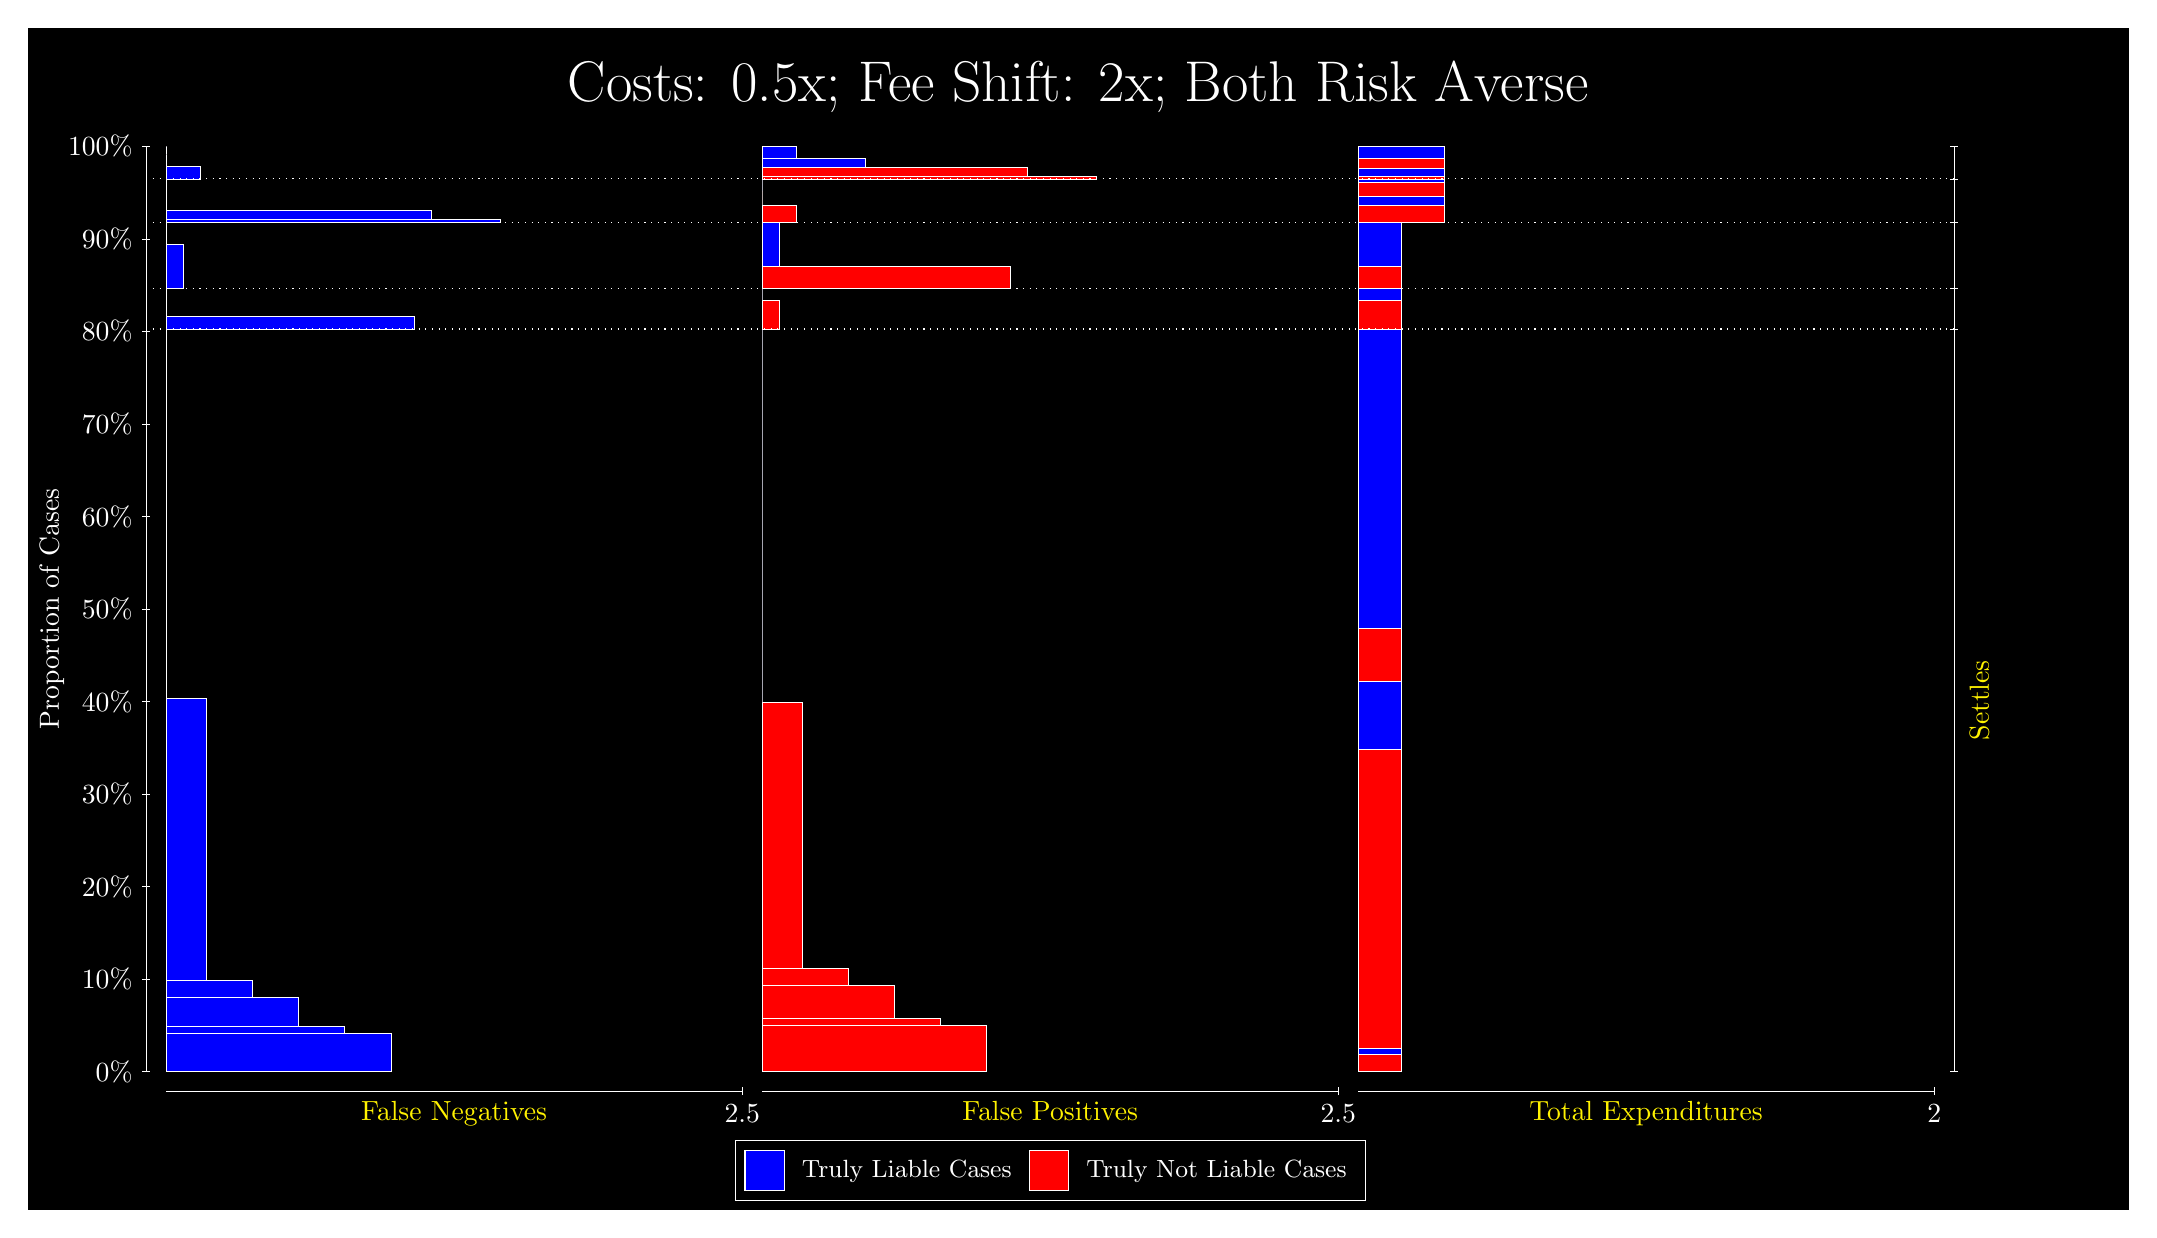
\begin{tikzpicture}
\draw[fill=black] (0,0) rectangle (26.667,15);
\draw[text=white] (0,13.5) rectangle (26.667,15) node[midway] {\huge Costs: 0.5x; Fee Shift: 2x; Both Risk Averse};
\draw[white, very thin] (1.5,1.75) -- (1.5,13.5);
\node[rotate=90, text=white, anchor=center] at (0.3, 7.625) {Proportion of Cases};
\draw[white, very thin] (1.45,1.75) -- (1.55,1.75);
\node[text=white, anchor=east] at (1.45, 1.75) {0\%};
\draw[white, very thin] (1.45,2.925) -- (1.55,2.925);
\node[text=white, anchor=east] at (1.45, 2.925) {10\%};
\draw[white, very thin] (1.45,4.1) -- (1.55,4.1);
\node[text=white, anchor=east] at (1.45, 4.1) {20\%};
\draw[white, very thin] (1.45,5.275) -- (1.55,5.275);
\node[text=white, anchor=east] at (1.45, 5.275) {30\%};
\draw[white, very thin] (1.45,6.45) -- (1.55,6.45);
\node[text=white, anchor=east] at (1.45, 6.45) {40\%};
\draw[white, very thin] (1.45,7.625) -- (1.55,7.625);
\node[text=white, anchor=east] at (1.45, 7.625) {50\%};
\draw[white, very thin] (1.45,8.8) -- (1.55,8.8);
\node[text=white, anchor=east] at (1.45, 8.8) {60\%};
\draw[white, very thin] (1.45,9.975) -- (1.55,9.975);
\node[text=white, anchor=east] at (1.45, 9.975) {70\%};
\draw[white, very thin] (1.45,11.15) -- (1.55,11.15);
\node[text=white, anchor=east] at (1.45, 11.15) {80\%};
\draw[white, very thin] (1.45,12.325) -- (1.55,12.325);
\node[text=white, anchor=east] at (1.45, 12.325) {90\%};
\draw[white, very thin] (1.45,13.5) -- (1.55,13.5);
\node[text=white, anchor=east] at (1.45, 13.5) {100\%};

\draw[white, very thin] (24.457,1.75) -- (24.457,13.5);
\draw[white, very thin] (24.407,1.75) -- (24.507,1.75);
\node[anchor=west] at (24.407, 1.75) {};
\draw[white, very thin] (24.407,11.18) -- (24.507,11.18);
\node[anchor=west] at (24.407, 11.18) {};
\draw[white, very thin] (24.407,11.698) -- (24.507,11.698);
\node[anchor=west] at (24.407, 11.698) {};
\draw[white, very thin] (24.407,12.535) -- (24.507,12.535);
\node[anchor=west] at (24.407, 12.535) {};
\draw[white, very thin] (24.407,13.086) -- (24.507,13.086);
\node[anchor=west] at (24.407, 13.086) {};
\draw[white, very thin] (24.407,13.5) -- (24.507,13.5);
\node[anchor=west] at (24.407, 13.5) {};

\draw[white, very thin, fill=blue] (1.75,1.75) rectangle (4.6044,2.2395);
\draw[white, very thin, fill=blue] (1.75,2.2395) rectangle (4.0188,2.3227);
\draw[white, very thin, fill=blue] (1.75,2.3227) rectangle (3.4333,2.6921);
\draw[white, very thin, fill=blue] (1.75,2.6921) rectangle (2.8478,2.9066);
\draw[white, very thin, fill=blue] (1.75,2.9066) rectangle (2.2623,6.4926);
\draw[white, very thin, fill=red] (1.75,6.4926) rectangle (1.75,11.18);
\draw[white, very thin, fill=blue] (1.75,11.18) rectangle (4.8971,11.336);
\draw[white, very thin, fill=red] (1.75,11.336) rectangle (1.75,11.698);
\draw[white, very thin, fill=blue] (1.75,11.698) rectangle (1.9696,12.259);
\draw[white, very thin, fill=red] (1.75,12.259) rectangle (1.75,12.535);
\draw[white, very thin, fill=blue] (1.75,12.535) rectangle (5.9949,12.575);
\draw[white, very thin, fill=blue] (1.75,12.575) rectangle (5.1167,12.69);
\draw[white, very thin, fill=red] (1.75,12.69) rectangle (1.75,13.086);
\draw[white, very thin, fill=blue] (1.75,13.086) rectangle (2.1891,13.244);
\draw[white, very thin, fill=red] (1.75,13.244) rectangle (1.75,13.398);
\draw[white, very thin, fill=blue] (1.75,13.398) rectangle (1.75,13.5);
\draw[white, very thin, fill=red] (9.3189,1.75) rectangle (12.173,2.3416);
\draw[white, very thin, fill=red] (9.3189,2.3416) rectangle (11.588,2.4249);
\draw[white, very thin, fill=red] (9.3189,2.4249) rectangle (11.002,2.8499);
\draw[white, very thin, fill=red] (9.3189,2.8499) rectangle (10.417,3.0644);
\draw[white, very thin, fill=red] (9.3189,3.0644) rectangle (9.8312,6.4371);
\draw[white, very thin, fill=blue] (9.3189,6.4371) rectangle (9.3189,11.18);
\draw[white, very thin, fill=red] (9.3189,11.18) rectangle (9.5384,11.541);
\draw[white, very thin, fill=blue] (9.3189,11.541) rectangle (9.3189,11.698);
\draw[white, very thin, fill=red] (9.3189,11.698) rectangle (12.466,11.973);
\draw[white, very thin, fill=blue] (9.3189,11.973) rectangle (9.5384,12.535);
\draw[white, very thin, fill=red] (9.3189,12.535) rectangle (9.758,12.753);
\draw[white, very thin, fill=red] (9.3189,12.753) rectangle (9.3189,12.932);
\draw[white, very thin, fill=blue] (9.3189,12.932) rectangle (9.3189,13.086);
\draw[white, very thin, fill=red] (9.3189,13.086) rectangle (13.564,13.118);
\draw[white, very thin, fill=red] (9.3189,13.118) rectangle (12.686,13.24);
\draw[white, very thin, fill=blue] (9.3189,13.24) rectangle (10.636,13.343);
\draw[white, very thin, fill=blue] (9.3189,13.343) rectangle (9.758,13.5);
\draw[white, very thin, fill=red] (16.888,1.75) rectangle (17.437,1.9646);
\draw[white, very thin, fill=blue] (16.888,1.9646) rectangle (17.437,2.0478);
\draw[white, very thin, fill=red] (16.888,2.0478) rectangle (17.437,5.8455);
\draw[white, very thin, fill=blue] (16.888,5.8455) rectangle (17.437,6.7044);
\draw[white, very thin, fill=red] (16.888,6.7044) rectangle (17.437,7.3793);
\draw[white, very thin, fill=blue] (16.888,7.3793) rectangle (17.437,11.18);
\draw[white, very thin, fill=red] (16.888,11.18) rectangle (17.437,11.541);
\draw[white, very thin, fill=blue] (16.888,11.541) rectangle (17.437,11.698);
\draw[white, very thin, fill=red] (16.888,11.698) rectangle (17.437,11.973);
\draw[white, very thin, fill=blue] (16.888,11.973) rectangle (17.437,12.535);
\draw[white, very thin, fill=red] (16.888,12.535) rectangle (17.986,12.753);
\draw[white, very thin, fill=blue] (16.888,12.753) rectangle (17.986,12.868);
\draw[white, very thin, fill=red] (16.888,12.868) rectangle (17.986,13.047);
\draw[white, very thin, fill=blue] (16.888,13.047) rectangle (17.986,13.086);
\draw[white, very thin, fill=red] (16.888,13.086) rectangle (17.986,13.118);
\draw[white, very thin, fill=blue] (16.888,13.118) rectangle (17.986,13.221);
\draw[white, very thin, fill=red] (16.888,13.221) rectangle (17.986,13.343);
\draw[white, very thin, fill=blue] (16.888,13.343) rectangle (17.986,13.5);
\draw[white, dotted] (1.5,11.18) -- (24.457,11.18);
\draw[white, dotted] (1.5,11.698) -- (24.457,11.698);
\draw[white, dotted] (1.5,12.535) -- (24.457,12.535);
\draw[white, dotted] (1.5,13.086) -- (24.457,13.086);
\draw[white, very thin] (1.75,1.5) -- (9.0689,1.5);
\node[text=yellow, anchor=north] at (5.4094, 1.5) {False Negatives};
\draw[white, very thin] (9.0689,1.45) -- (9.0689,1.55);
\node[text=white, anchor=north] at (9.0689, 1.45) {2.5};

\draw[white, very thin] (9.3189,1.5) -- (16.638,1.5);
\node[text=yellow, anchor=north] at (12.978, 1.5) {False Positives};
\draw[white, very thin] (16.638,1.45) -- (16.638,1.55);
\node[text=white, anchor=north] at (16.638, 1.45) {2.5};

\draw[white, very thin] (16.888,1.5) -- (24.207,1.5);
\node[text=yellow, anchor=north] at (20.547, 1.5) {Total Expenditures};
\draw[white, very thin] (24.207,1.45) -- (24.207,1.55);
\node[text=white, anchor=north] at (24.207, 1.45) {2};

\node[text=yellow, centered, rotate=90] at (24.777, 6.4649) {Settles};





\draw (12.978300999999998,1.5) node[draw=none] (baseCoordinate) {};
\begin{scope}[align=center]
        \matrix[scale=0.5, draw=white, below=0.5cm of baseCoordinate, nodes={draw}, column sep=0.1cm]{
            \node[rectangle, draw, minimum width=0.5cm, minimum height=0.5cm, fill=blue] {}; &
            \node[draw=none, font=\small, text=white] (B) {Truly Liable Cases}; &
            \node[rectangle, draw, minimum width=0.5cm, minimum height=0.5cm, fill=red] {}; &
            \node[draw=none, font=\small, text=white] (B) {Truly Not Liable Cases}; \\
            };
\end{scope}

\end{tikzpicture}
\end{document}